\section{Visión Artificial} \label{sect:Vision_Artificial}

Concepto Vision de computadoras (IMPORTANTE). En la inteligencia artificial es importante el reconocimiento de patrones y clasificación de objetos. El reconocimiento de objetos tiene como
objetivo la extracción de información en una imagen y la interpretación de la misma, a través de un proceso algorítmico.

\subsection{Filtros }
El filtrado de imágenes es una técnica para la transformación de imágenes, que consiste en destacar  sus características más relevantes orientadas a un propósito en particular. 

Generalmente en la tarea de extracción de información de una imagen se utilizan filtros para descartar zonas o características que no son importantes para el patrón deseado y para determinar el área deseada ya sea por patrones de forma o color.

En la investigación, los algoritmos de filtrado aplicados a las imágenes fueron: Clausura Morfológica y Apertura Morfológica, filtros que aplican las técnicas de erosión y dilatación a las imágenes.

\subsection{Transformaciones Morfológicas}
Las transformaciones morfológicas básicas son llamadas dilatación y erosión, y si Image Morphology que se presentan en una amplia variedad de contextos como la eliminación del ruido, aislamiento de elementos individuales, elementos de unión dispares en en una imagen.\cite{BookOpenCv}

\subsubsection{Dilatación}
La dilatación es una convulsión de alguna imagen (o región de una imagen) , que llamaremos A, con un núcleo que llamaremos B, el núcleo que puede ser de cualquier forma o tamaño, tiene un solo punto de anclaje definido. Muy  a menudo, el núcleo es un pequeño cuadrado o disco sólido con el punto de anclaje en el centro. El núcleo puede ser pensado como una plantilla  o mascarilla, y su efecto es que para la dilatación de un operador de máximo local sobre la imagen, se calcula el valor de píxel máximo común a B y reemplazamos el píxel de la imagen en el punto de anclaje con ese valor máximo. Esto causa regiones brillantes dentro de una imagen y la hacen crecer. Este crecimiento es el origen del término "operador de dilatación". \cite{BookOpenCv}

\begin{figure}[hbtp]
\caption{Dilatacion}
\centering
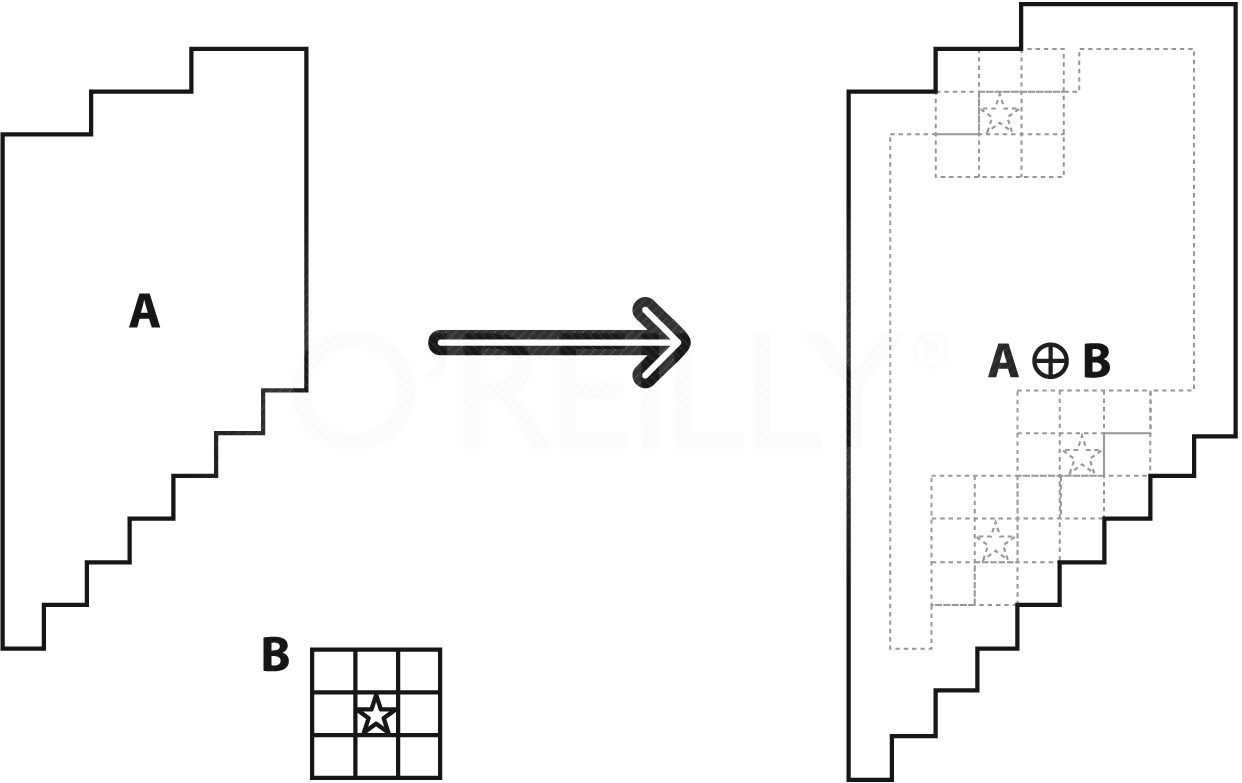
\includegraphics[scale=0.3]{imagenes/erosion-model.png}
\end{figure}


\subsubsection{Erosión}
La erosión es la operación inversa a la dilatación. Esta acción del operador es equivalente a la erosión el cálculo de un mínimo local sobre el área del núcleo. La erosión genera una nueva imagen desde la original, utilizando el siguiente algoritmo: como el núcleo B es analizado sobre la imagen, se calcula el mínimo valor del pixel superpuesto por B y se reemplaza el pixel de la imagen con un punto de anclaje de valor mínimo. \cite{BookOpenCv}

\begin{figure}[hbtp]
\caption{Erosion}
\centering
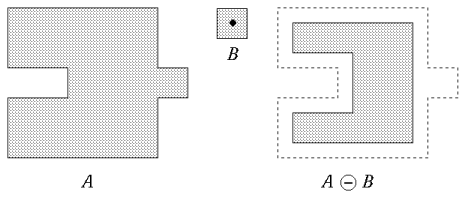
\includegraphics[scale=1]{imagenes/erosion.png}
\end{figure}
